\documentclass[1p]{elsarticle_modified}
%\bibliographystyle{elsarticle-num}

%\usepackage[colorlinks]{hyperref}
%\usepackage{abbrmath_seonhwa} %\Abb, \Ascr, \Acal ,\Abf, \Afrak
\usepackage{amsfonts}
\usepackage{amssymb}
\usepackage{amsmath}
\usepackage{amsthm}
\usepackage{scalefnt}
\usepackage{amsbsy}
\usepackage{kotex}
\usepackage{caption}
\usepackage{subfig}
\usepackage{color}
\usepackage{graphicx}
\usepackage{xcolor} %% white, black, red, green, blue, cyan, magenta, yellow
\usepackage{float}
\usepackage{setspace}
\usepackage{hyperref}

\usepackage{tikz}
\usetikzlibrary{arrows}

\usepackage{multirow}
\usepackage{array} % fixed length table
\usepackage{hhline}

%%%%%%%%%%%%%%%%%%%%%
\makeatletter
\renewcommand*\env@matrix[1][\arraystretch]{%
	\edef\arraystretch{#1}%
	\hskip -\arraycolsep
	\let\@ifnextchar\new@ifnextchar
	\array{*\c@MaxMatrixCols c}}
\makeatother %https://tex.stackexchange.com/questions/14071/how-can-i-increase-the-line-spacing-in-a-matrix
%%%%%%%%%%%%%%%

\usepackage[normalem]{ulem}

\newcommand{\msout}[1]{\ifmmode\text{\sout{\ensuremath{#1}}}\else\sout{#1}\fi}
%SOURCE: \msout is \stkout macro in https://tex.stackexchange.com/questions/20609/strikeout-in-math-mode

\newcommand{\cancel}[1]{
	\ifmmode
	{\color{red}\msout{#1}}
	\else
	{\color{red}\sout{#1}}
	\fi
}

\newcommand{\add}[1]{
	{\color{blue}\uwave{#1}}
}

\newcommand{\replace}[2]{
	\ifmmode
	{\color{red}\msout{#1}}{\color{blue}\uwave{#2}}
	\else
	{\color{red}\sout{#1}}{\color{blue}\uwave{#2}}
	\fi
}

\newcommand{\Sol}{\mathcal{S}} %segment
\newcommand{\D}{D} %diagram
\newcommand{\A}{\mathcal{A}} %arc


%%%%%%%%%%%%%%%%%%%%%%%%%%%%%5 test

\def\sl{\operatorname{\textup{SL}}(2,\Cbb)}
\def\psl{\operatorname{\textup{PSL}}(2,\Cbb)}
\def\quan{\mkern 1mu \triangleright \mkern 1mu}

\theoremstyle{definition}
\newtheorem{thm}{Theorem}[section]
\newtheorem{prop}[thm]{Proposition}
\newtheorem{lem}[thm]{Lemma}
\newtheorem{ques}[thm]{Question}
\newtheorem{cor}[thm]{Corollary}
\newtheorem{defn}[thm]{Definition}
\newtheorem{exam}[thm]{Example}
\newtheorem{rmk}[thm]{Remark}
\newtheorem{alg}[thm]{Algorithm}

\newcommand{\I}{\sqrt{-1}}
\begin{document}

%\begin{frontmatter}
%
%\title{Boundary parabolic representations of knots up to 8 crossings}
%
%%% Group authors per affiliation:
%\author{Yunhi Cho} 
%\address{Department of Mathematics, University of Seoul, Seoul, Korea}
%\ead{yhcho@uos.ac.kr}
%
%
%\author{Seonhwa Kim} %\fnref{s_kim}}
%\address{Center for Geometry and Physics, Institute for Basic Science, Pohang, 37673, Korea}
%\ead{ryeona17@ibs.re.kr}
%
%\author{Hyuk Kim}
%\address{Department of Mathematical Sciences, Seoul National University, Seoul 08826, Korea}
%\ead{hyukkim@snu.ac.kr}
%
%\author{Seokbeom Yoon}
%\address{Department of Mathematical Sciences, Seoul National University, Seoul, 08826,  Korea}
%\ead{sbyoon15@snu.ac.kr}
%
%\begin{abstract}
%We find all boundary parabolic representation of knots up to 8 crossings.
%
%\end{abstract}
%\begin{keyword}
%    \MSC[2010] 57M25 
%\end{keyword}
%
%\end{frontmatter}

%\linenumbers
%\tableofcontents
%
\newcommand\colored[1]{\textcolor{white}{\rule[-0.35ex]{0.8em}{1.4ex}}\kern-0.8em\color{red} #1}%
%\newcommand\colored[1]{\textcolor{white}{ #1}\kern-2.17ex	\textcolor{white}{ #1}\kern-1.81ex	\textcolor{white}{ #1}\kern-2.15ex\color{red}#1	}

{\Large $\underline{12a_{0590}~(K12a_{0590})}$}

\setlength{\tabcolsep}{10pt}
\renewcommand{\arraystretch}{1.6}
\vspace{1cm}\begin{tabular}{m{100pt}>{\centering\arraybackslash}m{274pt}}
\multirow{5}{120pt}{
	\centering
	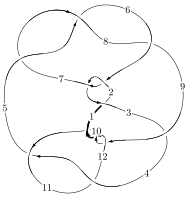
\includegraphics[width=112pt]{../../../GIT/diagram.site/Diagrams/png/1391_12a_0590.png}\\
\ \ \ A knot diagram\footnotemark}&
\allowdisplaybreaks
\textbf{Linearized knot diagam} \\
\cline{2-2}
 &
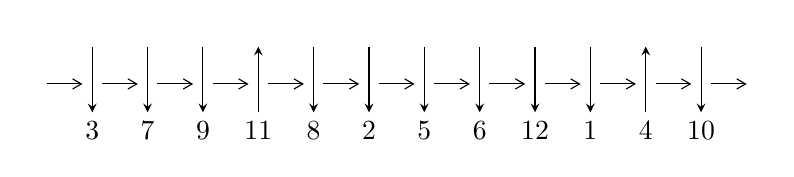
\begin{tikzpicture}[x=20pt, y=17pt]
	% nodes
	\node (C0) at (0, 0) {};
	\node (C1) at (1, 0) {};
	\node (C1U) at (1, +1) {};
	\node (C1D) at (1, -1) {3};

	\node (C2) at (2, 0) {};
	\node (C2U) at (2, +1) {};
	\node (C2D) at (2, -1) {7};

	\node (C3) at (3, 0) {};
	\node (C3U) at (3, +1) {};
	\node (C3D) at (3, -1) {9};

	\node (C4) at (4, 0) {};
	\node (C4U) at (4, +1) {};
	\node (C4D) at (4, -1) {11};

	\node (C5) at (5, 0) {};
	\node (C5U) at (5, +1) {};
	\node (C5D) at (5, -1) {8};

	\node (C6) at (6, 0) {};
	\node (C6U) at (6, +1) {};
	\node (C6D) at (6, -1) {2};

	\node (C7) at (7, 0) {};
	\node (C7U) at (7, +1) {};
	\node (C7D) at (7, -1) {5};

	\node (C8) at (8, 0) {};
	\node (C8U) at (8, +1) {};
	\node (C8D) at (8, -1) {6};

	\node (C9) at (9, 0) {};
	\node (C9U) at (9, +1) {};
	\node (C9D) at (9, -1) {12};

	\node (C10) at (10, 0) {};
	\node (C10U) at (10, +1) {};
	\node (C10D) at (10, -1) {1};

	\node (C11) at (11, 0) {};
	\node (C11U) at (11, +1) {};
	\node (C11D) at (11, -1) {4};

	\node (C12) at (12, 0) {};
	\node (C12U) at (12, +1) {};
	\node (C12D) at (12, -1) {10};
	\node (C13) at (13, 0) {};

	% arrows
	\draw[->,>={angle 60}]
	(C0) edge (C1) (C1) edge (C2) (C2) edge (C3) (C3) edge (C4) (C4) edge (C5) (C5) edge (C6) (C6) edge (C7) (C7) edge (C8) (C8) edge (C9) (C9) edge (C10) (C10) edge (C11) (C11) edge (C12) (C12) edge (C13) ;	\draw[->,>=stealth]
	(C1U) edge (C1D) (C2U) edge (C2D) (C3U) edge (C3D) (C4D) edge (C4U) (C5U) edge (C5D) (C6U) edge (C6D) (C7U) edge (C7D) (C8U) edge (C8D) (C9U) edge (C9D) (C10U) edge (C10D) (C11D) edge (C11U) (C12U) edge (C12D) ;
	\end{tikzpicture} \\
\hhline{~~} \\& 
\textbf{Solving Sequence} \\ \cline{2-2} 
 &
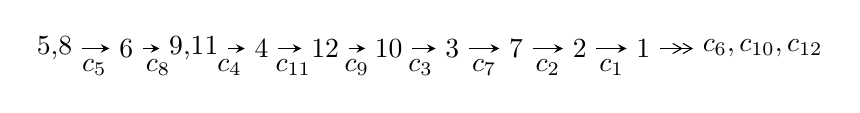
\begin{tikzpicture}[x=23pt, y=7pt]
	% node
	\node (A0) at (-1/8, 0) {5,8};
	\node (A1) at (1, 0) {6};
	\node (A2) at (33/16, 0) {9,11};
	\node (A3) at (25/8, 0) {4};
	\node (A4) at (33/8, 0) {12};
	\node (A5) at (41/8, 0) {10};
	\node (A6) at (49/8, 0) {3};
	\node (A7) at (57/8, 0) {7};
	\node (A8) at (65/8, 0) {2};
	\node (A9) at (73/8, 0) {1};
	\node (C1) at (1/2, -1) {$c_{5}$};
	\node (C2) at (3/2, -1) {$c_{8}$};
	\node (C3) at (21/8, -1) {$c_{4}$};
	\node (C4) at (29/8, -1) {$c_{11}$};
	\node (C5) at (37/8, -1) {$c_{9}$};
	\node (C6) at (45/8, -1) {$c_{3}$};
	\node (C7) at (53/8, -1) {$c_{7}$};
	\node (C8) at (61/8, -1) {$c_{2}$};
	\node (C9) at (69/8, -1) {$c_{1}$};
	\node (A10) at (11, 0) {$c_{6},c_{10},c_{12}$};

	% edge
	\draw[->,>=stealth]	
	(A0) edge (A1) (A1) edge (A2) (A2) edge (A3) (A3) edge (A4) (A4) edge (A5) (A5) edge (A6) (A6) edge (A7) (A7) edge (A8) (A8) edge (A9) ;
	\draw[->>,>={angle 60}]	
	(A9) edge (A10);
\end{tikzpicture} \\ 

\end{tabular} \\

\footnotetext{
The image of knot diagram is generated by the software ``\textbf{Draw programme}" developed by Andrew Bartholomew(\url{http://www.layer8.co.uk/maths/draw/index.htm\#Running-draw}), where we modified some parts for our purpose(\url{https://github.com/CATsTAILs/LinksPainter}).
}\phantom \\ \newline 
\centering \textbf{Ideals for irreducible components\footnotemark of $X_{\text{par}}$} 
 
\begin{align*}
I^u_{1}&=\langle 
1.68464\times10^{28} u^{87}+9.72953\times10^{28} u^{86}+\cdots+7.00197\times10^{26} b+1.37834\times10^{28},\\
\phantom{I^u_{1}}&\phantom{= \langle  }-1.24196\times10^{28} u^{87}-9.51690\times10^{28} u^{86}+\cdots+1.40039\times10^{27} a-3.17252\times10^{28},\;u^{88}+7 u^{87}+\cdots-5 u+1\rangle \\
I^u_{2}&=\langle 
b,\;u^7+2 u^6-2 u^5-4 u^4+2 u^3+u^2+a- u+3,\;u^8+u^7-3 u^6-2 u^5+3 u^4+2 u-1\rangle \\
I^u_{3}&=\langle 
a^4- a^3+a^2+b-2 a+1,\;a^5- a^4+a^3-2 a^2+a-1,\;u-1\rangle \\
\\
\end{align*}
\raggedright * 3 irreducible components of $\dim_{\mathbb{C}}=0$, with total 101 representations.\\
\footnotetext{All coefficients of polynomials are rational numbers. But the coefficients are sometimes approximated in decimal forms when there is not enough margin.}
\newpage
\renewcommand{\arraystretch}{1}
\centering \section*{I. $I^u_{1}= \langle 1.68\times10^{28} u^{87}+9.73\times10^{28} u^{86}+\cdots+7.00\times10^{26} b+1.38\times10^{28},\;-1.24\times10^{28} u^{87}-9.52\times10^{28} u^{86}+\cdots+1.40\times10^{27} a-3.17\times10^{28},\;u^{88}+7 u^{87}+\cdots-5 u+1 \rangle$}
\flushleft \textbf{(i) Arc colorings}\\
\begin{tabular}{m{7pt} m{180pt} m{7pt} m{180pt} }
\flushright $a_{5}=$&$\begin{pmatrix}1\\0\end{pmatrix}$ \\
\flushright $a_{8}=$&$\begin{pmatrix}0\\u\end{pmatrix}$ \\
\flushright $a_{6}=$&$\begin{pmatrix}1\\u^2\end{pmatrix}$ \\
\flushright $a_{9}=$&$\begin{pmatrix}- u\\- u^3+u\end{pmatrix}$ \\
\flushright $a_{11}=$&$\begin{pmatrix}8.86862 u^{87}+67.9587 u^{86}+\cdots-105.878 u+22.6545\\-24.0595 u^{87}-138.954 u^{86}+\cdots+110.889 u-19.6850\end{pmatrix}$ \\
\flushright $a_{4}=$&$\begin{pmatrix}25.3526 u^{87}+133.819 u^{86}+\cdots-76.7949 u+11.9623\\89.2486 u^{87}+498.120 u^{86}+\cdots-348.549 u+61.5438\end{pmatrix}$ \\
\flushright $a_{12}=$&$\begin{pmatrix}-17.3831 u^{87}-77.2993 u^{86}+\cdots-14.1162 u+6.54485\\-73.5892 u^{87}-406.913 u^{86}+\cdots+271.995 u-48.9600\end{pmatrix}$ \\
\flushright $a_{10}=$&$\begin{pmatrix}24.9048 u^{87}+121.952 u^{86}+\cdots-30.6185 u-0.170725\\107.854 u^{87}+601.429 u^{86}+\cdots-418.226 u+74.6075\end{pmatrix}$ \\
\flushright $a_{3}=$&$\begin{pmatrix}110.590 u^{87}+613.566 u^{86}+\cdots-427.222 u+73.2837\\162.309 u^{87}+914.917 u^{86}+\cdots-667.930 u+117.137\end{pmatrix}$ \\
\flushright $a_{7}=$&$\begin{pmatrix}u\\u\end{pmatrix}$ \\
\flushright $a_{2}=$&$\begin{pmatrix}177.819 u^{87}+1015.19 u^{86}+\cdots-782.351 u+133.966\\229.538 u^{87}+1316.54 u^{86}+\cdots-1023.06 u+177.819\end{pmatrix}$ \\
\flushright $a_{1}=$&$\begin{pmatrix}17.8946 u^{87}+106.795 u^{86}+\cdots-102.627 u+15.4769\\61.3214 u^{87}+344.013 u^{86}+\cdots-248.957 u+43.8200\end{pmatrix}$\\&\end{tabular}
\flushleft \textbf{(ii) Obstruction class $= -1$}\\~\\
\flushleft \textbf{(iii) Cusp Shapes $= -\frac{3994510142988588901229060665}{700197468586696191749097992} u^{87}-\frac{42648575021416709506457400371}{700197468586696191749097992} u^{86}+\cdots+\frac{107123801345113766348171177997}{700197468586696191749097992} u-\frac{4216109697287061694606989229}{175049367146674047937274498}$}\\~\\
\newpage\renewcommand{\arraystretch}{1}
\flushleft \textbf{(iv) u-Polynomials at the component}\newline \\
\begin{tabular}{m{50pt}|m{274pt}}
Crossings & \hspace{64pt}u-Polynomials at each crossing \\
\hline $$\begin{aligned}c_{1}\end{aligned}$$&$\begin{aligned}
&u^{88}+36 u^{87}+\cdots+16896 u+1024
\end{aligned}$\\
\hline $$\begin{aligned}c_{2},c_{6}\end{aligned}$$&$\begin{aligned}
&u^{88}-2 u^{87}+\cdots+64 u-32
\end{aligned}$\\
\hline $$\begin{aligned}c_{3}\end{aligned}$$&$\begin{aligned}
&u^{88}-3 u^{87}+\cdots+49703 u-30649
\end{aligned}$\\
\hline $$\begin{aligned}c_{4},c_{11}\end{aligned}$$&$\begin{aligned}
&u^{88}-2 u^{87}+\cdots-1664 u-256
\end{aligned}$\\
\hline $$\begin{aligned}c_{5},c_{7},c_{8}\end{aligned}$$&$\begin{aligned}
&u^{88}-7 u^{87}+\cdots+5 u+1
\end{aligned}$\\
\hline $$\begin{aligned}c_{9},c_{10},c_{12}\end{aligned}$$&$\begin{aligned}
&u^{88}-10 u^{87}+\cdots-13 u+1
\end{aligned}$\\
\hline
\end{tabular}\\~\\
\newpage\renewcommand{\arraystretch}{1}
\flushleft \textbf{(v) Riley Polynomials at the component}\newline \\
\begin{tabular}{m{50pt}|m{274pt}}
Crossings & \hspace{64pt}Riley Polynomials at each crossing \\
\hline $$\begin{aligned}c_{1}\end{aligned}$$&$\begin{aligned}
&y^{88}+24 y^{87}+\cdots-10092544 y+1048576
\end{aligned}$\\
\hline $$\begin{aligned}c_{2},c_{6}\end{aligned}$$&$\begin{aligned}
&y^{88}-36 y^{87}+\cdots-16896 y+1024
\end{aligned}$\\
\hline $$\begin{aligned}c_{3}\end{aligned}$$&$\begin{aligned}
&y^{88}-37 y^{87}+\cdots-880685877 y+939361201
\end{aligned}$\\
\hline $$\begin{aligned}c_{4},c_{11}\end{aligned}$$&$\begin{aligned}
&y^{88}+54 y^{87}+\cdots-49152 y+65536
\end{aligned}$\\
\hline $$\begin{aligned}c_{5},c_{7},c_{8}\end{aligned}$$&$\begin{aligned}
&y^{88}-77 y^{87}+\cdots-7 y+1
\end{aligned}$\\
\hline $$\begin{aligned}c_{9},c_{10},c_{12}\end{aligned}$$&$\begin{aligned}
&y^{88}-86 y^{87}+\cdots-85 y+1
\end{aligned}$\\
\hline
\end{tabular}\\~\\
\newpage\flushleft \textbf{(vi) Complex Volumes and Cusp Shapes}
$$\begin{array}{c|c|c}  
\text{Solutions to }I^u_{1}& \I (\text{vol} + \sqrt{-1}CS) & \text{Cusp shape}\\
 \hline 
\begin{aligned}
u &= \phantom{-}0.888121 + 0.465628 I \\
a &= -0.674944 - 0.581430 I \\
b &= \phantom{-}1.115510 - 0.134578 I\end{aligned}
 & -5.34037 + 0.66509 I & \phantom{-0.000000 } 0 \\ \hline\begin{aligned}
u &= \phantom{-}0.888121 - 0.465628 I \\
a &= -0.674944 + 0.581430 I \\
b &= \phantom{-}1.115510 + 0.134578 I\end{aligned}
 & -5.34037 - 0.66509 I & \phantom{-0.000000 } 0 \\ \hline\begin{aligned}
u &= \phantom{-}0.766339 + 0.598583 I \\
a &= -1.036980 - 0.856681 I \\
b &= \phantom{-}0.42193 - 1.40540 I\end{aligned}
 & -10.41430 - 4.71583 I & \phantom{-0.000000 } 0 \\ \hline\begin{aligned}
u &= \phantom{-}0.766339 - 0.598583 I \\
a &= -1.036980 + 0.856681 I \\
b &= \phantom{-}0.42193 + 1.40540 I\end{aligned}
 & -10.41430 + 4.71583 I & \phantom{-0.000000 } 0 \\ \hline\begin{aligned}
u &= \phantom{-}0.952850 + 0.465179 I \\
a &= -0.065021 - 0.913422 I \\
b &= -0.351118 - 1.102560 I\end{aligned}
 & -2.96134 + 2.94865 I & \phantom{-0.000000 } 0 \\ \hline\begin{aligned}
u &= \phantom{-}0.952850 - 0.465179 I \\
a &= -0.065021 + 0.913422 I \\
b &= -0.351118 + 1.102560 I\end{aligned}
 & -2.96134 - 2.94865 I & \phantom{-0.000000 } 0 \\ \hline\begin{aligned}
u &= \phantom{-}0.800920 + 0.458340 I \\
a &= \phantom{-}0.73265 + 1.28159 I \\
b &= -0.112227 + 1.047930 I\end{aligned}
 & -3.55064 - 1.70767 I & \phantom{-0.000000 } 0 \\ \hline\begin{aligned}
u &= \phantom{-}0.800920 - 0.458340 I \\
a &= \phantom{-}0.73265 - 1.28159 I \\
b &= -0.112227 - 1.047930 I\end{aligned}
 & -3.55064 + 1.70767 I & \phantom{-0.000000 } 0 \\ \hline\begin{aligned}
u &= \phantom{-}0.238802 + 0.874394 I \\
a &= -1.51165 - 0.29886 I \\
b &= \phantom{-}0.64367 - 1.34705 I\end{aligned}
 & -6.87264 - 11.71080 I & \phantom{-0.000000 } 0 \\ \hline\begin{aligned}
u &= \phantom{-}0.238802 - 0.874394 I \\
a &= -1.51165 + 0.29886 I \\
b &= \phantom{-}0.64367 + 1.34705 I\end{aligned}
 & -6.87264 + 11.71080 I & \phantom{-0.000000 } 0\\
 \hline 
 \end{array}$$\newpage$$\begin{array}{c|c|c}  
\text{Solutions to }I^u_{1}& \I (\text{vol} + \sqrt{-1}CS) & \text{Cusp shape}\\
 \hline 
\begin{aligned}
u &= \phantom{-}1.106230 + 0.101887 I \\
a &= -0.38448 + 2.75149 I \\
b &= \phantom{-}0.253569 + 0.477806 I\end{aligned}
 & -3.31594 - 0.58556 I & \phantom{-0.000000 } 0 \\ \hline\begin{aligned}
u &= \phantom{-}1.106230 - 0.101887 I \\
a &= -0.38448 - 2.75149 I \\
b &= \phantom{-}0.253569 - 0.477806 I\end{aligned}
 & -3.31594 + 0.58556 I & \phantom{-0.000000 } 0 \\ \hline\begin{aligned}
u &= \phantom{-}1.074860 + 0.294544 I \\
a &= \phantom{-}0.609880 + 0.504609 I \\
b &= -0.493783 + 0.368228 I\end{aligned}
 & -0.723913 - 0.558805 I & \phantom{-0.000000 } 0 \\ \hline\begin{aligned}
u &= \phantom{-}1.074860 - 0.294544 I \\
a &= \phantom{-}0.609880 - 0.504609 I \\
b &= -0.493783 - 0.368228 I\end{aligned}
 & -0.723913 + 0.558805 I & \phantom{-0.000000 } 0 \\ \hline\begin{aligned}
u &= \phantom{-}0.998684 + 0.532410 I \\
a &= \phantom{-}0.123794 + 0.448994 I \\
b &= \phantom{-}0.58280 + 1.35034 I\end{aligned}
 & -9.19064 + 6.74935 I & \phantom{-0.000000 } 0 \\ \hline\begin{aligned}
u &= \phantom{-}0.998684 - 0.532410 I \\
a &= \phantom{-}0.123794 - 0.448994 I \\
b &= \phantom{-}0.58280 - 1.35034 I\end{aligned}
 & -9.19064 - 6.74935 I & \phantom{-0.000000 } 0 \\ \hline\begin{aligned}
u &= \phantom{-}0.394607 + 0.770272 I \\
a &= \phantom{-}0.455783 + 0.010772 I \\
b &= \phantom{-}0.31689 + 1.42777 I\end{aligned}
 & -9.29942 - 0.08924 I & \phantom{-0.000000 } 0 \\ \hline\begin{aligned}
u &= \phantom{-}0.394607 - 0.770272 I \\
a &= \phantom{-}0.455783 - 0.010772 I \\
b &= \phantom{-}0.31689 - 1.42777 I\end{aligned}
 & -9.29942 + 0.08924 I & \phantom{-0.000000 } 0 \\ \hline\begin{aligned}
u &= \phantom{-}0.236702 + 0.827946 I \\
a &= \phantom{-}1.33516 + 0.60966 I \\
b &= -0.428462 + 1.161060 I\end{aligned}
 & -0.75062 - 7.56823 I & \phantom{-0.000000 } 0 \\ \hline\begin{aligned}
u &= \phantom{-}0.236702 - 0.827946 I \\
a &= \phantom{-}1.33516 - 0.60966 I \\
b &= -0.428462 - 1.161060 I\end{aligned}
 & -0.75062 + 7.56823 I & \phantom{-0.000000 } 0\\
 \hline 
 \end{array}$$\newpage$$\begin{array}{c|c|c}  
\text{Solutions to }I^u_{1}& \I (\text{vol} + \sqrt{-1}CS) & \text{Cusp shape}\\
 \hline 
\begin{aligned}
u &= \phantom{-}0.257930 + 0.804225 I \\
a &= -0.992899 - 0.708956 I \\
b &= \phantom{-}1.176510 + 0.257378 I\end{aligned}
 & -3.37075 - 5.18603 I & \phantom{-0.000000 } 0 \\ \hline\begin{aligned}
u &= \phantom{-}0.257930 - 0.804225 I \\
a &= -0.992899 + 0.708956 I \\
b &= \phantom{-}1.176510 - 0.257378 I\end{aligned}
 & -3.37075 + 5.18603 I & \phantom{-0.000000 } 0 \\ \hline\begin{aligned}
u &= \phantom{-}0.044598 + 0.812501 I \\
a &= \phantom{-}0.012409 - 0.949891 I \\
b &= -0.068037 + 0.976812 I\end{aligned}
 & -0.94317 - 2.91824 I & -8.00000 + 0. I\phantom{ +0.000000I} \\ \hline\begin{aligned}
u &= \phantom{-}0.044598 - 0.812501 I \\
a &= \phantom{-}0.012409 + 0.949891 I \\
b &= -0.068037 - 0.976812 I\end{aligned}
 & -0.94317 + 2.91824 I & -8.00000 + 0. I\phantom{ +0.000000I} \\ \hline\begin{aligned}
u &= \phantom{-}0.265848 + 0.760527 I \\
a &= -0.709338 - 0.763779 I \\
b &= \phantom{-}0.074648 - 1.085590 I\end{aligned}
 & -1.85509 - 2.57254 I & \phantom{-0.000000 } 0 \\ \hline\begin{aligned}
u &= \phantom{-}0.265848 - 0.760527 I \\
a &= -0.709338 + 0.763779 I \\
b &= \phantom{-}0.074648 + 1.085590 I\end{aligned}
 & -1.85509 + 2.57254 I & \phantom{-0.000000 } 0 \\ \hline\begin{aligned}
u &= \phantom{-}0.164802 + 0.765395 I \\
a &= \phantom{-}0.640282 + 0.424932 I \\
b &= -0.640037 - 0.265485 I\end{aligned}
 & \phantom{-}1.98407 - 3.37950 I & -3.18324 + 4.49505 I \\ \hline\begin{aligned}
u &= \phantom{-}0.164802 - 0.765395 I \\
a &= \phantom{-}0.640282 - 0.424932 I \\
b &= -0.640037 + 0.265485 I\end{aligned}
 & \phantom{-}1.98407 + 3.37950 I & -3.18324 - 4.49505 I \\ \hline\begin{aligned}
u &= -1.210690 + 0.142812 I \\
a &= \phantom{-}0.167563 + 0.494552 I \\
b &= -0.564547 + 1.141500 I\end{aligned}
 & -8.03151 - 3.54347 I & \phantom{-0.000000 } 0 \\ \hline\begin{aligned}
u &= -1.210690 - 0.142812 I \\
a &= \phantom{-}0.167563 - 0.494552 I \\
b &= -0.564547 - 1.141500 I\end{aligned}
 & -8.03151 + 3.54347 I & \phantom{-0.000000 } 0\\
 \hline 
 \end{array}$$\newpage$$\begin{array}{c|c|c}  
\text{Solutions to }I^u_{1}& \I (\text{vol} + \sqrt{-1}CS) & \text{Cusp shape}\\
 \hline 
\begin{aligned}
u &= \phantom{-}1.239120 + 0.245897 I \\
a &= \phantom{-}0.512434 - 0.571361 I \\
b &= \phantom{-}0.566252 + 0.257444 I\end{aligned}
 & -1.10788 - 1.71772 I & \phantom{-0.000000 } 0 \\ \hline\begin{aligned}
u &= \phantom{-}1.239120 - 0.245897 I \\
a &= \phantom{-}0.512434 + 0.571361 I \\
b &= \phantom{-}0.566252 - 0.257444 I\end{aligned}
 & -1.10788 + 1.71772 I & \phantom{-0.000000 } 0 \\ \hline\begin{aligned}
u &= \phantom{-}1.215600 + 0.383630 I \\
a &= -0.934428 - 0.097206 I \\
b &= \phantom{-}0.033207 - 1.038470 I\end{aligned}
 & -4.54745 - 1.38520 I & \phantom{-0.000000 } 0 \\ \hline\begin{aligned}
u &= \phantom{-}1.215600 - 0.383630 I \\
a &= -0.934428 + 0.097206 I \\
b &= \phantom{-}0.033207 + 1.038470 I\end{aligned}
 & -4.54745 + 1.38520 I & \phantom{-0.000000 } 0 \\ \hline\begin{aligned}
u &= -1.276630 + 0.183299 I \\
a &= -0.215638 - 0.758974 I \\
b &= \phantom{-}0.582952 - 0.942243 I\end{aligned}
 & -2.95506 + 0.13185 I & \phantom{-0.000000 } 0 \\ \hline\begin{aligned}
u &= -1.276630 - 0.183299 I \\
a &= -0.215638 + 0.758974 I \\
b &= \phantom{-}0.582952 + 0.942243 I\end{aligned}
 & -2.95506 - 0.13185 I & \phantom{-0.000000 } 0 \\ \hline\begin{aligned}
u &= \phantom{-}0.051522 + 0.675391 I \\
a &= -0.742113 + 0.645879 I \\
b &= \phantom{-}0.611315 - 0.427751 I\end{aligned}
 & \phantom{-}2.51572 - 1.61584 I & -1.91976 + 3.16837 I \\ \hline\begin{aligned}
u &= \phantom{-}0.051522 - 0.675391 I \\
a &= -0.742113 - 0.645879 I \\
b &= \phantom{-}0.611315 + 0.427751 I\end{aligned}
 & \phantom{-}2.51572 + 1.61584 I & -1.91976 - 3.16837 I \\ \hline\begin{aligned}
u &= \phantom{-}1.314380 + 0.174281 I \\
a &= \phantom{-}1.09840 + 2.65275 I \\
b &= \phantom{-}0.010805 + 1.079500 I\end{aligned}
 & -4.65633 - 0.63571 I & \phantom{-0.000000 } 0 \\ \hline\begin{aligned}
u &= \phantom{-}1.314380 - 0.174281 I \\
a &= \phantom{-}1.09840 - 2.65275 I \\
b &= \phantom{-}0.010805 - 1.079500 I\end{aligned}
 & -4.65633 + 0.63571 I & \phantom{-0.000000 } 0\\
 \hline 
 \end{array}$$\newpage$$\begin{array}{c|c|c}  
\text{Solutions to }I^u_{1}& \I (\text{vol} + \sqrt{-1}CS) & \text{Cusp shape}\\
 \hline 
\begin{aligned}
u &= -1.320720 + 0.187553 I \\
a &= \phantom{-}0.655900 - 0.911111 I \\
b &= -0.908877 - 0.545626 I\end{aligned}
 & -6.01527 + 1.89183 I & \phantom{-0.000000 } 0 \\ \hline\begin{aligned}
u &= -1.320720 - 0.187553 I \\
a &= \phantom{-}0.655900 + 0.911111 I \\
b &= -0.908877 + 0.545626 I\end{aligned}
 & -6.01527 - 1.89183 I & \phantom{-0.000000 } 0 \\ \hline\begin{aligned}
u &= -1.307460 + 0.264842 I \\
a &= -0.436161 + 0.563621 I \\
b &= \phantom{-}0.704898 + 0.536481 I\end{aligned}
 & -1.74045 + 5.01419 I & \phantom{-0.000000 } 0 \\ \hline\begin{aligned}
u &= -1.307460 - 0.264842 I \\
a &= -0.436161 - 0.563621 I \\
b &= \phantom{-}0.704898 - 0.536481 I\end{aligned}
 & -1.74045 - 5.01419 I & \phantom{-0.000000 } 0 \\ \hline\begin{aligned}
u &= -1.292640 + 0.344864 I \\
a &= \phantom{-}0.615494 - 0.130607 I \\
b &= -0.165716 - 0.926745 I\end{aligned}
 & -5.11018 + 7.07530 I & \phantom{-0.000000 } 0 \\ \hline\begin{aligned}
u &= -1.292640 - 0.344864 I \\
a &= \phantom{-}0.615494 + 0.130607 I \\
b &= -0.165716 + 0.926745 I\end{aligned}
 & -5.11018 - 7.07530 I & \phantom{-0.000000 } 0 \\ \hline\begin{aligned}
u &= -0.174131 + 0.636836 I \\
a &= \phantom{-}2.02360 - 0.48082 I \\
b &= -0.580461 - 1.285720 I\end{aligned}
 & -5.14037 + 6.25877 I & -9.44624 - 3.66252 I \\ \hline\begin{aligned}
u &= -0.174131 - 0.636836 I \\
a &= \phantom{-}2.02360 + 0.48082 I \\
b &= -0.580461 + 1.285720 I\end{aligned}
 & -5.14037 - 6.25877 I & -9.44624 + 3.66252 I \\ \hline\begin{aligned}
u &= \phantom{-}1.330870 + 0.207803 I \\
a &= -0.933904 + 0.972883 I \\
b &= -1.166170 - 0.198096 I\end{aligned}
 & -6.30741 - 3.16964 I & \phantom{-0.000000 } 0 \\ \hline\begin{aligned}
u &= \phantom{-}1.330870 - 0.207803 I \\
a &= -0.933904 - 0.972883 I \\
b &= -1.166170 + 0.198096 I\end{aligned}
 & -6.30741 + 3.16964 I & \phantom{-0.000000 } 0\\
 \hline 
 \end{array}$$\newpage$$\begin{array}{c|c|c}  
\text{Solutions to }I^u_{1}& \I (\text{vol} + \sqrt{-1}CS) & \text{Cusp shape}\\
 \hline 
\begin{aligned}
u &= \phantom{-}1.332230 + 0.235913 I \\
a &= -1.36376 - 2.55428 I \\
b &= \phantom{-}0.386394 - 1.149300 I\end{aligned}
 & -3.80107 - 5.54437 I & \phantom{-0.000000 } 0 \\ \hline\begin{aligned}
u &= \phantom{-}1.332230 - 0.235913 I \\
a &= -1.36376 + 2.55428 I \\
b &= \phantom{-}0.386394 + 1.149300 I\end{aligned}
 & -3.80107 + 5.54437 I & \phantom{-0.000000 } 0 \\ \hline\begin{aligned}
u &= -1.339550 + 0.224805 I \\
a &= \phantom{-}0.091229 + 1.306420 I \\
b &= -0.487922 + 0.888767 I\end{aligned}
 & -5.42509 + 4.45293 I & \phantom{-0.000000 } 0 \\ \hline\begin{aligned}
u &= -1.339550 - 0.224805 I \\
a &= \phantom{-}0.091229 - 1.306420 I \\
b &= -0.487922 - 0.888767 I\end{aligned}
 & -5.42509 - 4.45293 I & \phantom{-0.000000 } 0 \\ \hline\begin{aligned}
u &= \phantom{-}1.380100 + 0.123580 I \\
a &= -1.09435 - 2.36932 I \\
b &= -0.37266 - 1.42969 I\end{aligned}
 & -11.86110 + 2.15849 I & \phantom{-0.000000 } 0 \\ \hline\begin{aligned}
u &= \phantom{-}1.380100 - 0.123580 I \\
a &= -1.09435 + 2.36932 I \\
b &= -0.37266 + 1.42969 I\end{aligned}
 & -11.86110 - 2.15849 I & \phantom{-0.000000 } 0 \\ \hline\begin{aligned}
u &= \phantom{-}1.365220 + 0.261535 I \\
a &= \phantom{-}1.33626 + 2.41346 I \\
b &= -0.61664 + 1.35909 I\end{aligned}
 & -10.02730 - 9.55714 I & \phantom{-0.000000 } 0 \\ \hline\begin{aligned}
u &= \phantom{-}1.365220 - 0.261535 I \\
a &= \phantom{-}1.33626 - 2.41346 I \\
b &= -0.61664 - 1.35909 I\end{aligned}
 & -10.02730 + 9.55714 I & \phantom{-0.000000 } 0 \\ \hline\begin{aligned}
u &= -1.363890 + 0.319129 I \\
a &= -0.234330 - 0.481461 I \\
b &= -0.705464 + 0.206220 I\end{aligned}
 & -2.84821 + 7.30244 I & \phantom{-0.000000 } 0 \\ \hline\begin{aligned}
u &= -1.363890 - 0.319129 I \\
a &= -0.234330 + 0.481461 I \\
b &= -0.705464 - 0.206220 I\end{aligned}
 & -2.84821 - 7.30244 I & \phantom{-0.000000 } 0\\
 \hline 
 \end{array}$$\newpage$$\begin{array}{c|c|c}  
\text{Solutions to }I^u_{1}& \I (\text{vol} + \sqrt{-1}CS) & \text{Cusp shape}\\
 \hline 
\begin{aligned}
u &= -1.40144\phantom{ +0.000000I} \\
a &= -0.385644\phantom{ +0.000000I} \\
b &= -0.577672\phantom{ +0.000000I}\end{aligned}
 & -7.10454\phantom{ +0.000000I} & \phantom{-0.000000 } 0 \\ \hline\begin{aligned}
u &= -0.087677 + 0.585925 I \\
a &= -1.96671 + 0.65542 I \\
b &= \phantom{-}0.433173 + 1.031780 I\end{aligned}
 & \phantom{-}0.69910 + 2.52777 I & -5.84354 - 3.35799 I \\ \hline\begin{aligned}
u &= -0.087677 - 0.585925 I \\
a &= -1.96671 - 0.65542 I \\
b &= \phantom{-}0.433173 - 1.031780 I\end{aligned}
 & \phantom{-}0.69910 - 2.52777 I & -5.84354 + 3.35799 I \\ \hline\begin{aligned}
u &= \phantom{-}0.563116\phantom{ +0.000000I} \\
a &= \phantom{-}0.509143\phantom{ +0.000000I} \\
b &= -0.313068\phantom{ +0.000000I}\end{aligned}
 & -0.958674\phantom{ +0.000000I} & -9.85690\phantom{ +0.000000I} \\ \hline\begin{aligned}
u &= -1.40715 + 0.30877 I \\
a &= -0.99962 + 1.99298 I \\
b &= \phantom{-}0.120608 + 1.188840 I\end{aligned}
 & -7.16857 + 6.45126 I & \phantom{-0.000000 } 0 \\ \hline\begin{aligned}
u &= -1.40715 - 0.30877 I \\
a &= -0.99962 - 1.99298 I \\
b &= \phantom{-}0.120608 - 1.188840 I\end{aligned}
 & -7.16857 - 6.45126 I & \phantom{-0.000000 } 0 \\ \hline\begin{aligned}
u &= \phantom{-}0.124503 + 0.544345 I \\
a &= \phantom{-}1.27598 - 0.81112 I \\
b &= -0.260698 - 0.771913 I\end{aligned}
 & -0.80366 - 1.58561 I & -10.67225 + 2.90476 I \\ \hline\begin{aligned}
u &= \phantom{-}0.124503 - 0.544345 I \\
a &= \phantom{-}1.27598 + 0.81112 I \\
b &= -0.260698 + 0.771913 I\end{aligned}
 & -0.80366 + 1.58561 I & -10.67225 - 2.90476 I \\ \hline\begin{aligned}
u &= -1.40680 + 0.34051 I \\
a &= \phantom{-}1.26967 - 1.96871 I \\
b &= -0.455387 - 1.216770 I\end{aligned}
 & -5.97118 + 11.78330 I & \phantom{-0.000000 } 0 \\ \hline\begin{aligned}
u &= -1.40680 - 0.34051 I \\
a &= \phantom{-}1.26967 + 1.96871 I \\
b &= -0.455387 + 1.216770 I\end{aligned}
 & -5.97118 - 11.78330 I & \phantom{-0.000000 } 0\\
 \hline 
 \end{array}$$\newpage$$\begin{array}{c|c|c}  
\text{Solutions to }I^u_{1}& \I (\text{vol} + \sqrt{-1}CS) & \text{Cusp shape}\\
 \hline 
\begin{aligned}
u &= -1.41173 + 0.32636 I \\
a &= \phantom{-}0.451797 + 0.801134 I \\
b &= \phantom{-}1.251800 - 0.295347 I\end{aligned}
 & -8.68021 + 9.27069 I & \phantom{-0.000000 } 0 \\ \hline\begin{aligned}
u &= -1.41173 - 0.32636 I \\
a &= \phantom{-}0.451797 - 0.801134 I \\
b &= \phantom{-}1.251800 + 0.295347 I\end{aligned}
 & -8.68021 - 9.27069 I & \phantom{-0.000000 } 0 \\ \hline\begin{aligned}
u &= -1.41652 + 0.36230 I \\
a &= -1.32614 + 1.85531 I \\
b &= \phantom{-}0.68460 + 1.36460 I\end{aligned}
 & -12.1310 + 16.1617 I & \phantom{-0.000000 } 0 \\ \hline\begin{aligned}
u &= -1.41652 - 0.36230 I \\
a &= -1.32614 - 1.85531 I \\
b &= \phantom{-}0.68460 - 1.36460 I\end{aligned}
 & -12.1310 - 16.1617 I & \phantom{-0.000000 } 0 \\ \hline\begin{aligned}
u &= -1.45238 + 0.27357 I \\
a &= \phantom{-}0.98226 - 1.57277 I \\
b &= \phantom{-}0.26475 - 1.52039 I\end{aligned}
 & -15.2401 + 3.8156 I & \phantom{-0.000000 } 0 \\ \hline\begin{aligned}
u &= -1.45238 - 0.27357 I \\
a &= \phantom{-}0.98226 + 1.57277 I \\
b &= \phantom{-}0.26475 + 1.52039 I\end{aligned}
 & -15.2401 - 3.8156 I & \phantom{-0.000000 } 0 \\ \hline\begin{aligned}
u &= -1.47888 + 0.02352 I \\
a &= \phantom{-}0.11238 - 2.43472 I \\
b &= -0.196285 - 1.246890 I\end{aligned}
 & -11.09960 + 2.70583 I & \phantom{-0.000000 } 0 \\ \hline\begin{aligned}
u &= -1.47888 - 0.02352 I \\
a &= \phantom{-}0.11238 + 2.43472 I \\
b &= -0.196285 + 1.246890 I\end{aligned}
 & -11.09960 - 2.70583 I & \phantom{-0.000000 } 0 \\ \hline\begin{aligned}
u &= -1.48451\phantom{ +0.000000I} \\
a &= \phantom{-}0.899695\phantom{ +0.000000I} \\
b &= \phantom{-}1.29707\phantom{ +0.000000I}\end{aligned}
 & -13.2474\phantom{ +0.000000I} & \phantom{-0.000000 } 0 \\ \hline\begin{aligned}
u &= -0.051131 + 0.501827 I \\
a &= \phantom{-}1.30705 - 1.31645 I \\
b &= -0.963746 + 0.258016 I\end{aligned}
 & -1.87492 + 0.52113 I & -7.46007 + 0.33584 I\\
 \hline 
 \end{array}$$\newpage$$\begin{array}{c|c|c}  
\text{Solutions to }I^u_{1}& \I (\text{vol} + \sqrt{-1}CS) & \text{Cusp shape}\\
 \hline 
\begin{aligned}
u &= -0.051131 - 0.501827 I \\
a &= \phantom{-}1.30705 + 1.31645 I \\
b &= -0.963746 - 0.258016 I\end{aligned}
 & -1.87492 - 0.52113 I & -7.46007 - 0.33584 I \\ \hline\begin{aligned}
u &= -1.51084 + 0.06009 I \\
a &= -0.09053 + 2.25061 I \\
b &= \phantom{-}0.52441 + 1.48832 I\end{aligned}
 & -18.1852 + 6.5334 I & \phantom{-0.000000 } 0 \\ \hline\begin{aligned}
u &= -1.51084 - 0.06009 I \\
a &= -0.09053 - 2.25061 I \\
b &= \phantom{-}0.52441 - 1.48832 I\end{aligned}
 & -18.1852 - 6.5334 I & \phantom{-0.000000 } 0 \\ \hline\begin{aligned}
u &= -0.346736 + 0.293540 I \\
a &= -1.47471 + 0.88660 I \\
b &= -0.407022 + 1.274040 I\end{aligned}
 & -6.45539 - 3.75624 I & -8.92208 + 2.37124 I \\ \hline\begin{aligned}
u &= -0.346736 - 0.293540 I \\
a &= -1.47471 - 0.88660 I \\
b &= -0.407022 - 1.274040 I\end{aligned}
 & -6.45539 + 3.75624 I & -8.92208 - 2.37124 I \\ \hline\begin{aligned}
u &= -0.109910 + 0.191162 I \\
a &= \phantom{-}2.62502 - 1.00223 I \\
b &= \phantom{-}0.221171 - 0.788369 I\end{aligned}
 & -0.464107 - 1.212900 I & -5.34512 + 5.07325 I \\ \hline\begin{aligned}
u &= -0.109910 - 0.191162 I \\
a &= \phantom{-}2.62502 + 1.00223 I \\
b &= \phantom{-}0.221171 + 0.788369 I\end{aligned}
 & -0.464107 + 1.212900 I & -5.34512 - 5.07325 I \\ \hline\begin{aligned}
u &= \phantom{-}0.164075\phantom{ +0.000000I} \\
a &= \phantom{-}6.48224\phantom{ +0.000000I} \\
b &= -0.479550\phantom{ +0.000000I}\end{aligned}
 & -2.12876\phantom{ +0.000000I} & -0.110400\phantom{ +0.000000I}\\
 \hline 
 \end{array}$$\newpage\newpage\renewcommand{\arraystretch}{1}
\centering \section*{II. $I^u_{2}= \langle b,\;u^7+2 u^6-2 u^5-4 u^4+2 u^3+u^2+a- u+3,\;u^8+u^7-3 u^6-2 u^5+3 u^4+2 u-1 \rangle$}
\flushleft \textbf{(i) Arc colorings}\\
\begin{tabular}{m{7pt} m{180pt} m{7pt} m{180pt} }
\flushright $a_{5}=$&$\begin{pmatrix}1\\0\end{pmatrix}$ \\
\flushright $a_{8}=$&$\begin{pmatrix}0\\u\end{pmatrix}$ \\
\flushright $a_{6}=$&$\begin{pmatrix}1\\u^2\end{pmatrix}$ \\
\flushright $a_{9}=$&$\begin{pmatrix}- u\\- u^3+u\end{pmatrix}$ \\
\flushright $a_{11}=$&$\begin{pmatrix}- u^7-2 u^6+2 u^5+4 u^4-2 u^3- u^2+u-3\\0\end{pmatrix}$ \\
\flushright $a_{4}=$&$\begin{pmatrix}1\\0\end{pmatrix}$ \\
\flushright $a_{12}=$&$\begin{pmatrix}- u^7-2 u^6+2 u^5+4 u^4-2 u^3- u^2+u-3\\0\end{pmatrix}$ \\
\flushright $a_{10}=$&$\begin{pmatrix}- u^7-2 u^6+2 u^5+4 u^4-2 u^3- u^2-3\\- u^3+u\end{pmatrix}$ \\
\flushright $a_{3}=$&$\begin{pmatrix}- u^4+u^2+1\\- u^6+2 u^4- u^2\end{pmatrix}$ \\
\flushright $a_{7}=$&$\begin{pmatrix}u\\u\end{pmatrix}$ \\
\flushright $a_{2}=$&$\begin{pmatrix}u^7-2 u^5+2 u\\u^7- u^6-2 u^5+3 u^4-2 u^2+2 u-1\end{pmatrix}$ \\
\flushright $a_{1}=$&$\begin{pmatrix}u\\u^3- u\end{pmatrix}$\\&\end{tabular}
\flushleft \textbf{(ii) Obstruction class $= 1$}\\~\\
\flushleft \textbf{(iii) Cusp Shapes $= -3 u^7-10 u^6+7 u^5+25 u^4-9 u^3-12 u^2+8 u-25$}\\~\\
\newpage\renewcommand{\arraystretch}{1}
\flushleft \textbf{(iv) u-Polynomials at the component}\newline \\
\begin{tabular}{m{50pt}|m{274pt}}
Crossings & \hspace{64pt}u-Polynomials at each crossing \\
\hline $$\begin{aligned}c_{1},c_{3}\end{aligned}$$&$\begin{aligned}
&u^8-3 u^7+7 u^6-10 u^5+11 u^4-10 u^3+6 u^2-4 u+1
\end{aligned}$\\
\hline $$\begin{aligned}c_{2}\end{aligned}$$&$\begin{aligned}
&u^8- u^7- u^6+2 u^5+u^4-2 u^3+2 u-1
\end{aligned}$\\
\hline $$\begin{aligned}c_{4},c_{11}\end{aligned}$$&$\begin{aligned}
&u^8
\end{aligned}$\\
\hline $$\begin{aligned}c_{5}\end{aligned}$$&$\begin{aligned}
&u^8+u^7-3 u^6-2 u^5+3 u^4+2 u-1
\end{aligned}$\\
\hline $$\begin{aligned}c_{6}\end{aligned}$$&$\begin{aligned}
&u^8+u^7- u^6-2 u^5+u^4+2 u^3-2 u-1
\end{aligned}$\\
\hline $$\begin{aligned}c_{7},c_{8}\end{aligned}$$&$\begin{aligned}
&u^8- u^7-3 u^6+2 u^5+3 u^4-2 u-1
\end{aligned}$\\
\hline $$\begin{aligned}c_{9},c_{10}\end{aligned}$$&$\begin{aligned}
&(u-1)^8
\end{aligned}$\\
\hline $$\begin{aligned}c_{12}\end{aligned}$$&$\begin{aligned}
&(u+1)^8
\end{aligned}$\\
\hline
\end{tabular}\\~\\
\newpage\renewcommand{\arraystretch}{1}
\flushleft \textbf{(v) Riley Polynomials at the component}\newline \\
\begin{tabular}{m{50pt}|m{274pt}}
Crossings & \hspace{64pt}Riley Polynomials at each crossing \\
\hline $$\begin{aligned}c_{1},c_{3}\end{aligned}$$&$\begin{aligned}
&y^8+5 y^7+11 y^6+6 y^5-17 y^4-34 y^3-22 y^2-4 y+1
\end{aligned}$\\
\hline $$\begin{aligned}c_{2},c_{6}\end{aligned}$$&$\begin{aligned}
&y^8-3 y^7+7 y^6-10 y^5+11 y^4-10 y^3+6 y^2-4 y+1
\end{aligned}$\\
\hline $$\begin{aligned}c_{4},c_{11}\end{aligned}$$&$\begin{aligned}
&y^8
\end{aligned}$\\
\hline $$\begin{aligned}c_{5},c_{7},c_{8}\end{aligned}$$&$\begin{aligned}
&y^8-7 y^7+19 y^6-22 y^5+3 y^4+14 y^3-6 y^2-4 y+1
\end{aligned}$\\
\hline $$\begin{aligned}c_{9},c_{10},c_{12}\end{aligned}$$&$\begin{aligned}
&(y-1)^8
\end{aligned}$\\
\hline
\end{tabular}\\~\\
\newpage\flushleft \textbf{(vi) Complex Volumes and Cusp Shapes}
$$\begin{array}{c|c|c}  
\text{Solutions to }I^u_{2}& \I (\text{vol} + \sqrt{-1}CS) & \text{Cusp shape}\\
 \hline 
\begin{aligned}
u &= \phantom{-}1.180120 + 0.268597 I \\
a &= \phantom{-}0.281371 - 1.128550 I \\
b &= \phantom{-0.000000 } 0\end{aligned}
 & -2.68559 - 1.13123 I & -9.56807 + 0.79885 I \\ \hline\begin{aligned}
u &= \phantom{-}1.180120 - 0.268597 I \\
a &= \phantom{-}0.281371 + 1.128550 I \\
b &= \phantom{-0.000000 } 0\end{aligned}
 & -2.68559 + 1.13123 I & -9.56807 - 0.79885 I \\ \hline\begin{aligned}
u &= \phantom{-}0.108090 + 0.747508 I \\
a &= -0.208670 + 0.825203 I \\
b &= \phantom{-0.000000 } 0\end{aligned}
 & \phantom{-}0.51448 - 2.57849 I & -6.42531 + 3.25625 I \\ \hline\begin{aligned}
u &= \phantom{-}0.108090 - 0.747508 I \\
a &= -0.208670 - 0.825203 I \\
b &= \phantom{-0.000000 } 0\end{aligned}
 & \phantom{-}0.51448 + 2.57849 I & -6.42531 - 3.25625 I \\ \hline\begin{aligned}
u &= -1.37100\phantom{ +0.000000I} \\
a &= -0.829189\phantom{ +0.000000I} \\
b &= \phantom{-0.000000 } 0\end{aligned}
 & -8.14766\phantom{ +0.000000I} & -20.0060\phantom{ +0.000000I} \\ \hline\begin{aligned}
u &= -1.334530 + 0.318930 I \\
a &= -0.284386 - 0.605794 I \\
b &= \phantom{-0.000000 } 0\end{aligned}
 & -4.02461 + 6.44354 I & -11.71592 - 3.92092 I \\ \hline\begin{aligned}
u &= -1.334530 - 0.318930 I \\
a &= -0.284386 + 0.605794 I \\
b &= \phantom{-0.000000 } 0\end{aligned}
 & -4.02461 - 6.44354 I & -11.71592 + 3.92092 I \\ \hline\begin{aligned}
u &= \phantom{-}0.463640\phantom{ +0.000000I} \\
a &= -2.74744\phantom{ +0.000000I} \\
b &= \phantom{-0.000000 } 0\end{aligned}
 & -2.48997\phantom{ +0.000000I} & -23.5750\phantom{ +0.000000I}\\
 \hline 
 \end{array}$$\newpage\newpage\renewcommand{\arraystretch}{1}
\centering \section*{III. $I^u_{3}= \langle a^4- a^3+a^2+b-2 a+1,\;a^5- a^4+a^3-2 a^2+a-1,\;u-1 \rangle$}
\flushleft \textbf{(i) Arc colorings}\\
\begin{tabular}{m{7pt} m{180pt} m{7pt} m{180pt} }
\flushright $a_{5}=$&$\begin{pmatrix}1\\0\end{pmatrix}$ \\
\flushright $a_{8}=$&$\begin{pmatrix}0\\1\end{pmatrix}$ \\
\flushright $a_{6}=$&$\begin{pmatrix}1\\1\end{pmatrix}$ \\
\flushright $a_{9}=$&$\begin{pmatrix}-1\\0\end{pmatrix}$ \\
\flushright $a_{11}=$&$\begin{pmatrix}a\\- a^4+a^3- a^2+2 a-1\end{pmatrix}$ \\
\flushright $a_{4}=$&$\begin{pmatrix}0\\a^4- a-1\end{pmatrix}$ \\
\flushright $a_{12}=$&$\begin{pmatrix}a\\- a^3+1\end{pmatrix}$ \\
\flushright $a_{10}=$&$\begin{pmatrix}a^4- a-1\\a^3- a^2-2\end{pmatrix}$ \\
\flushright $a_{3}=$&$\begin{pmatrix}a^4- a-1\\a^4- a-1\end{pmatrix}$ \\
\flushright $a_{7}=$&$\begin{pmatrix}1\\1\end{pmatrix}$ \\
\flushright $a_{2}=$&$\begin{pmatrix}a^4- a-1\\a^4- a-1\end{pmatrix}$ \\
\flushright $a_{1}=$&$\begin{pmatrix}a^4- a-1\\a^4- a-1\end{pmatrix}$\\&\end{tabular}
\flushleft \textbf{(ii) Obstruction class $= 1$}\\~\\
\flushleft \textbf{(iii) Cusp Shapes $= -5 a^4+5 a^3+7 a-14$}\\~\\
\newpage\renewcommand{\arraystretch}{1}
\flushleft \textbf{(iv) u-Polynomials at the component}\newline \\
\begin{tabular}{m{50pt}|m{274pt}}
Crossings & \hspace{64pt}u-Polynomials at each crossing \\
\hline $$\begin{aligned}c_{1},c_{2},c_{6}\end{aligned}$$&$\begin{aligned}
&u^5
\end{aligned}$\\
\hline $$\begin{aligned}c_{3}\end{aligned}$$&$\begin{aligned}
&u^5+3 u^4+4 u^3+u^2- u-1
\end{aligned}$\\
\hline $$\begin{aligned}c_{4}\end{aligned}$$&$\begin{aligned}
&u^5+u^4+2 u^3+u^2+u+1
\end{aligned}$\\
\hline $$\begin{aligned}c_{5}\end{aligned}$$&$\begin{aligned}
&(u-1)^5
\end{aligned}$\\
\hline $$\begin{aligned}c_{7},c_{8}\end{aligned}$$&$\begin{aligned}
&(u+1)^5
\end{aligned}$\\
\hline $$\begin{aligned}c_{9},c_{10}\end{aligned}$$&$\begin{aligned}
&u^5+u^4-2 u^3- u^2+u-1
\end{aligned}$\\
\hline $$\begin{aligned}c_{11}\end{aligned}$$&$\begin{aligned}
&u^5- u^4+2 u^3- u^2+u-1
\end{aligned}$\\
\hline $$\begin{aligned}c_{12}\end{aligned}$$&$\begin{aligned}
&u^5- u^4-2 u^3+u^2+u+1
\end{aligned}$\\
\hline
\end{tabular}\\~\\
\newpage\renewcommand{\arraystretch}{1}
\flushleft \textbf{(v) Riley Polynomials at the component}\newline \\
\begin{tabular}{m{50pt}|m{274pt}}
Crossings & \hspace{64pt}Riley Polynomials at each crossing \\
\hline $$\begin{aligned}c_{1},c_{2},c_{6}\end{aligned}$$&$\begin{aligned}
&y^5
\end{aligned}$\\
\hline $$\begin{aligned}c_{3}\end{aligned}$$&$\begin{aligned}
&y^5- y^4+8 y^3-3 y^2+3 y-1
\end{aligned}$\\
\hline $$\begin{aligned}c_{4},c_{11}\end{aligned}$$&$\begin{aligned}
&y^5+3 y^4+4 y^3+y^2- y-1
\end{aligned}$\\
\hline $$\begin{aligned}c_{5},c_{7},c_{8}\end{aligned}$$&$\begin{aligned}
&(y-1)^5
\end{aligned}$\\
\hline $$\begin{aligned}c_{9},c_{10},c_{12}\end{aligned}$$&$\begin{aligned}
&y^5-5 y^4+8 y^3-3 y^2- y-1
\end{aligned}$\\
\hline
\end{tabular}\\~\\
\newpage\flushleft \textbf{(vi) Complex Volumes and Cusp Shapes}
$$\begin{array}{c|c|c}  
\text{Solutions to }I^u_{3}& \I (\text{vol} + \sqrt{-1}CS) & \text{Cusp shape}\\
 \hline 
\begin{aligned}
u &= \phantom{-}1.00000\phantom{ +0.000000I} \\
a &= -0.428550 + 1.039280 I \\
b &= \phantom{-}0.339110 + 0.822375 I\end{aligned}
 & -1.97403 + 1.53058 I & -10.50099 - 3.45976 I \\ \hline\begin{aligned}
u &= \phantom{-}1.00000\phantom{ +0.000000I} \\
a &= -0.428550 - 1.039280 I \\
b &= \phantom{-}0.339110 - 0.822375 I\end{aligned}
 & -1.97403 - 1.53058 I & -10.50099 + 3.45976 I \\ \hline\begin{aligned}
u &= \phantom{-}1.00000\phantom{ +0.000000I} \\
a &= \phantom{-}0.276511 + 0.728237 I \\
b &= -0.455697 + 1.200150 I\end{aligned}
 & -7.51750 - 4.40083 I & -14.3774 + 5.8297 I \\ \hline\begin{aligned}
u &= \phantom{-}1.00000\phantom{ +0.000000I} \\
a &= \phantom{-}0.276511 - 0.728237 I \\
b &= -0.455697 - 1.200150 I\end{aligned}
 & -7.51750 + 4.40083 I & -14.3774 - 5.8297 I \\ \hline\begin{aligned}
u &= \phantom{-}1.00000\phantom{ +0.000000I} \\
a &= \phantom{-}1.30408\phantom{ +0.000000I} \\
b &= -0.766826\phantom{ +0.000000I}\end{aligned}
 & -4.04602\phantom{ +0.000000I} & -8.24330\phantom{ +0.000000I}\\
 \hline 
 \end{array}$$\newpage
\newpage\renewcommand{\arraystretch}{1}
\centering \section*{ IV. u-Polynomials}
\begin{tabular}{m{50pt}|m{274pt}}
Crossings & \hspace{64pt}u-Polynomials at each crossing \\
\hline $$\begin{aligned}c_{1}\end{aligned}$$&$\begin{aligned}
&u^5(u^8-3 u^7+7 u^6-10 u^5+11 u^4-10 u^3+6 u^2-4 u+1)\\
&\cdot(u^{88}+36 u^{87}+\cdots+16896 u+1024)
\end{aligned}$\\
\hline $$\begin{aligned}c_{2}\end{aligned}$$&$\begin{aligned}
&u^5(u^8- u^7+\cdots+2 u-1)(u^{88}-2 u^{87}+\cdots+64 u-32)
\end{aligned}$\\
\hline $$\begin{aligned}c_{3}\end{aligned}$$&$\begin{aligned}
&(u^5+3 u^4+4 u^3+u^2- u-1)\\
&\cdot(u^8-3 u^7+7 u^6-10 u^5+11 u^4-10 u^3+6 u^2-4 u+1)\\
&\cdot(u^{88}-3 u^{87}+\cdots+49703 u-30649)
\end{aligned}$\\
\hline $$\begin{aligned}c_{4}\end{aligned}$$&$\begin{aligned}
&u^8(u^5+u^4+\cdots+u+1)(u^{88}-2 u^{87}+\cdots-1664 u-256)
\end{aligned}$\\
\hline $$\begin{aligned}c_{5}\end{aligned}$$&$\begin{aligned}
&((u-1)^5)(u^8+u^7+\cdots+2 u-1)(u^{88}-7 u^{87}+\cdots+5 u+1)
\end{aligned}$\\
\hline $$\begin{aligned}c_{6}\end{aligned}$$&$\begin{aligned}
&u^5(u^8+u^7+\cdots-2 u-1)(u^{88}-2 u^{87}+\cdots+64 u-32)
\end{aligned}$\\
\hline $$\begin{aligned}c_{7},c_{8}\end{aligned}$$&$\begin{aligned}
&((u+1)^5)(u^8- u^7+\cdots-2 u-1)(u^{88}-7 u^{87}+\cdots+5 u+1)
\end{aligned}$\\
\hline $$\begin{aligned}c_{9},c_{10}\end{aligned}$$&$\begin{aligned}
&((u-1)^8)(u^5+u^4+\cdots+u-1)(u^{88}-10 u^{87}+\cdots-13 u+1)
\end{aligned}$\\
\hline $$\begin{aligned}c_{11}\end{aligned}$$&$\begin{aligned}
&u^8(u^5- u^4+\cdots+u-1)(u^{88}-2 u^{87}+\cdots-1664 u-256)
\end{aligned}$\\
\hline $$\begin{aligned}c_{12}\end{aligned}$$&$\begin{aligned}
&((u+1)^8)(u^5- u^4+\cdots+u+1)(u^{88}-10 u^{87}+\cdots-13 u+1)
\end{aligned}$\\
\hline
\end{tabular}\newpage\renewcommand{\arraystretch}{1}
\centering \section*{ V. Riley Polynomials}
\begin{tabular}{m{50pt}|m{274pt}}
Crossings & \hspace{64pt}Riley Polynomials at each crossing \\
\hline $$\begin{aligned}c_{1}\end{aligned}$$&$\begin{aligned}
&y^5(y^8+5 y^7+11 y^6+6 y^5-17 y^4-34 y^3-22 y^2-4 y+1)\\
&\cdot(y^{88}+24 y^{87}+\cdots-10092544 y+1048576)
\end{aligned}$\\
\hline $$\begin{aligned}c_{2},c_{6}\end{aligned}$$&$\begin{aligned}
&y^5(y^8-3 y^7+7 y^6-10 y^5+11 y^4-10 y^3+6 y^2-4 y+1)\\
&\cdot(y^{88}-36 y^{87}+\cdots-16896 y+1024)
\end{aligned}$\\
\hline $$\begin{aligned}c_{3}\end{aligned}$$&$\begin{aligned}
&(y^5- y^4+8 y^3-3 y^2+3 y-1)\\
&\cdot(y^8+5 y^7+11 y^6+6 y^5-17 y^4-34 y^3-22 y^2-4 y+1)\\
&\cdot(y^{88}-37 y^{87}+\cdots-880685877 y+939361201)
\end{aligned}$\\
\hline $$\begin{aligned}c_{4},c_{11}\end{aligned}$$&$\begin{aligned}
&y^8(y^5+3 y^4+\cdots- y-1)(y^{88}+54 y^{87}+\cdots-49152 y+65536)
\end{aligned}$\\
\hline $$\begin{aligned}c_{5},c_{7},c_{8}\end{aligned}$$&$\begin{aligned}
&(y-1)^5(y^8-7 y^7+19 y^6-22 y^5+3 y^4+14 y^3-6 y^2-4 y+1)\\
&\cdot(y^{88}-77 y^{87}+\cdots-7 y+1)
\end{aligned}$\\
\hline $$\begin{aligned}c_{9},c_{10},c_{12}\end{aligned}$$&$\begin{aligned}
&((y-1)^8)(y^5-5 y^4+\cdots- y-1)(y^{88}-86 y^{87}+\cdots-85 y+1)
\end{aligned}$\\
\hline
\end{tabular}
\vskip 2pc
\end{document}